\documentclass[12pt]{article}
\usepackage{multicol}
\usepackage{apacite}
\usepackage{graphicx}
\DeclareGraphicsExtensions{.pdf,.svg,.png,.jpg}

% title page
\begin{document}
\title{Visualizing and Refining Connectivity Map Query Results}
\maketitle
\begin{titlepage}
\begin{center}
Proposal for a\\
Thesis in the Field of\\
Biotechnology\\[\baselineskip]
In Partial Fulfillment of the Requirements\\
for a Master of Liberal Arts Degree\\[\baselineskip]
Harvard University\\
Extension School\\[\baselineskip]
Theodore Natoli\\
51 Lewis Avenue, Apartment 3\\
Arlington, MA 02472\\
857-498-1946\\
\texttt{tnatoli@fas.harvard.edu}\\[\baselineskip]
Proposed Start Date: \today\\
Anticipated Date of Graduation: \today\\
Thesis Director: Aravind Subramanian
\end{center}
\end{titlepage}
% end of title stuff

\begin{abstract}
The Connectivity Map (CMap) is a database of gene expression signatures obtained from experiments in which cultured human cells are treated with pharmacologic and genomic perturbagens. A typical use case of this database is for a researcher to query with a signature of a cell state of interest and use the matching perturbagens to develop a functional hypothesis for follow-up. 

Current pattern matching algorithms that perform CMap queries suffer from a universal weakness -- the enormous size and richness of signatures in CMap means that a query typically generates hundreds of strong correlations which are hard to distinguish thereby making prioritization on the basis of a distance metric difficult.

We hypothesize that one mode of prioritization is to highlight query results that are highly interconnected amongst themselves over singletons. The goal of this work is to provide a web-based tool for implementing an interconnectivity-based method of query result refinement and of visualizing CMap query results in a graph layout.
\end{abstract}


% background
\section{Background}
\subsection{The Connectivity Map}
The connectivity map is a database containing the gene expression profiles resulting from treating cultured cells with various chemical and genomic perturbations \cite{lamb2006}.
\subsection{Graphical Models}
\subsection{Graphical Depictions of Biological Phenomena}
Although they originated in the field of computer science, graphs have frequently been used as tools to model biological phenomena. Graphical models of protein interaction networks, gene expression networks, and other similar phenomena are commonplace. Because of its widespread use and adoption, I believe the graphical model is an appropriate and effective means to depict connectivity in the CMap sense.
\subsection{Approach for This Work}
In this work, a graph will be used to depict the existence and strength of connections between gene expression signatures in the CMap database. Signatures will be represented as nodes and their pairwise connections by the edges. The final app might look something like this.
% app mockup image
\begin{figure}[h]
\centering
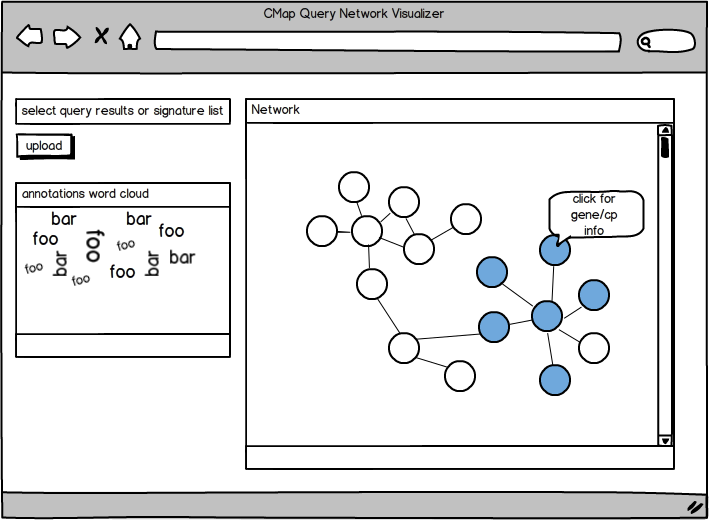
\includegraphics[scale=0.5]{img/app_mockup}
\caption{The App}
\label{fig:app_mockup}
\end{figure}

% methods
\section{Methods}
\subsection{Software Components}
\subsubsection{Front End: HTML \& D3.js}
\subsubsection{Back End: Node.js \& MongoDB}

% challenges
\section{Potential Challenges}



% timeline
\section{Preliminary Timeline}

% bibliography
\bibliographystyle{apacite}
\bibliography{bibliography}

\end{document}